%% Created on June 28th, 2010;
\documentclass[a4paper]{article}
\usepackage{geometry}
\usepackage{fancyhdr}
\usepackage{amsmath}
\usepackage{booktabs}
\usepackage{graphicx}
\usepackage{amsthm}
\usepackage{array}
\geometry{top=1.3in, bottom=1.3in, left=1.2in, right=1.2in}

% defs.
\newtheorem{simondef}{Definition}

% Start of doc.
\begin{document}

\title{Perceived and Realized Risk of Online Social Networks}

\maketitle

\begin{abstract}
With the fast development of Online Social Networks (OSN), privacy
issue has become a great concern. Privacy settings of OSN may involve
hundreds of items, indicating how the user presents himself/herself to
other users. Hiding or disclosing private information to other users
is basically a personal choice. However, disclosing private
information also comes with certain risks such as information spam,
insurance discrimination, and financial fraud. Meanwhile, people
disclose private information to gain some social benefits, such as
getting reconnected with old friends and open to job
opportunities. OSN users may implicitly make decision on privacy
disclosure based on a personal tradeoff between the risks and the
benefits. Is there a global pattern representing most users’ concern
about the implicit privacy risk? How to model the privacy risk in
terms of social network structure? How can users quantitatively
evaluate the privacy risks and social benefits by disclosing or hiding
a private item? In this paper, we mine real data from online social
network to investigate people’s feeling about the tradeoff between
privacy risk and social benefits of disclosing certain personal
information item. Either privacy risk or social benefit is realized
only when a certain profile item is visited by another OSN user. We
also model the probability of visit based on the user’s personal
social network structure and derive the expectation of realized
privacy risk. The social benefits can be modeled in a similar
way. These models can help users assess their privacy settings of
profile items according to potential benefits and risks.

\end{abstract}

% With the fast development of Online Social Networks (OSN), privacy
% issue has become a great concern. Among all the research attempts of
% social network privacy, quantification of OSN user risks is an
% important attempt to deal with this problem. But how to quantify the
% privacy risks faced by OSN users is a challenging problem. Past work
% on this topic has been done by Justin et
% al.\cite{measure-privacy-risk}, Tran Hong et
% al. \cite{SN-quantify-privacy} and Kun et
% al. \cite{SN-privacy-score}. Kun et al. proposed a model to calculate
% the privacy score of OSN users. The model uses two intuitive metrics,
% sensitivity and visibility, as the factors for privacy score
% calculation. Inspired by the work done by Kun et al., we propose a
% model to quantify the privacy risks of OSN users, our model assume
% that OSN users intent to enjoy the benefits of OSNs, but on the other
% hand, the disclosure of personal information also brings risks to the
% social network users which are potentially hidden.

% The social benefits is determined by the number of users who can view
% an item. The more viewer, the higher social benefit. On the other
% hand, the implied privacy risks by disclosing an item is determined by
% how sensitive the item is as well as the potential users. The
% networked environment of OSN determines the potential audiences of a
% profile item.

% And we argue that the privacy risk is also based on the probability
% that a certain profile item is visited by another OSN user. We model
% this probability as a random walk process over all the potential
% social network users.

% In summary, by integrating social benefits and potential risks, our
% model tells the relative privacy risks of social network users for
% specific profile setting.

\section{Introduction}
% background of social networks.
In recent years, online social networking is becoming a popular life
style for many users. [rewrite benefits of social networking, it
provides people a virtual world for social relations. In order to
enjoy these benefits, users have to disclose their personal
information to allow other users search, identify and link them.

% people are providing their personal
% information to enjoy the benefits of these social sites. While, on the
% other hand, the risks of privacy breach through social network becomes
% and urgent and a more and more of public concern.

% privacy risks caused by using of social networks.
Disclosing private information also raises certain risks such as
information spam \cite{}, insurance discrimination \cite{}, and
finacial fraud \cite{identity-theft-attack}. \textbf{[some examples
show how malicious parties can use the private information to damage
users' interests.]  To be added later} These examples may educate
people how risk to disclose personal information. People are more and
more aware of the risk of disclosing private information. As a result,
hiding or disclosing a profile item is a personal tradeoff between
privacy risks and social benefits.

% [the following examples are not about the risk of disclosing private
% information. They represent the importance of taking users' privacy
% concern into system design. ]

% And several social network accidents also tells the truth of privacy
% risks of online social networks. Years ago, facebook's
% Beacon\cite{facebook-turnoff-beacon}, which correlate users' shopping
% activities on other websites with their Facebook profiles, had to be
% closed because of the protests of users' personal privacy
% violation. Google buzz\cite{googlebuzz}, a social networking,
% microblogging and 
% messaging tool from Google integrated into Gmail, was sued because of
% compromising users' privacy by sharing their email contacts to
% maximize influence of this service. These and other similar social
% network privacy breach incidents have educated people to have more
% concern on the privacy of their private information, for example, they
% may ask\cite{user_privacy}, what benefits and risks can I have if I
% disclose my personal information on the social network? And people are
% unwilling to risk losing control of their personal information.

Intuitively, different personal information items may be associated
with different levels of risk. To make this tradeoff between risks and
benefits, people may want to know what the level of risk is if they
disclose a personal information item. Although people understand more
and more private-information based attacks, it is difficult to
quantitively evaluate the level of risk and rank the profile items by
the damages caused by disclosing them. A comprehensive approach is to
understand all the possible attacks that utilize the exposed personal
information and then evaluate the overall damages of disclosing a
profile item. We refer the privacy risk defined by this approach as
\emph{real privacy risk}, which is our long-term goal.

Alternatively, it is also useful to learn what people feel about
privacy risks. The hypothesis is that most people have taken the risk
factors into consideration when they adjust their privacy
settings. The aggregated user opinions about privacy setting of a
profile item could provide some clues about the level of risk of this
item. We name the aggregated user judgement as the \emph{perceived
  privacy risk}.

The privacy risk is not \emph{realized}, if the profile item is not
seen by another user. We argue that the probability of a profile item
is seen is determined by the user's privacy setting and the structure
of his/her social network. Therefore, we also study how network
structure affects the realized privacy risk.

In this paper, we study the perceived privacy risk with real facebook
data and build a model for estimating the expectation of realized
privacy risk. This paper has three unique contributions.
\begin{itemize}
\item We believe that privacy setting of social network profile items
  is not only a personal preference, but also related to the risks
  associated with exposing the specific profile items. A better
  understanding of the privacy risk can be built around the concepts
  such as real privacy risks, perceived privacy risk, and realized
  privacy risk.

\item We propose an empirical method to study users' implicit
  judgements on the privacy risk, with which we can guide new users of
  social networks or existing users unaware of privacy risks to
  evaluate their privacy settings.

\item We propose a network based model fro estimating the expected
  realized privacy risk. With this model and the privacy risk measure
  (either real or perceived), a user can estimate the potential
  privacy risk by disclosing one specific item to different levels of
  audience.
\end{itemize}

%% what is our model of privacy score and our contributions.
% In this paper, we are making attempt to answer this particular
% question, to quantify the benefits and risks of engaging in social
% networks. Without loss of generality, we use Facebook as our main
% target for analysis. Similar models can be extend to other social
% networks.

% We argue that the main driving force for people to join in a social
% network is the benefit provided by such networks, and the disclosure
% of personal sensitive information to social networks poses privacy
% risks which is negative from a user's point of view. We try to
% integrate these two together and define privacy as combination of
% positive social network benefits as well as negative social network
% privacy risks.

% We define privacy as a probablistic problem , which considers user as
% in a network and privacy risks happens when the user is visited by
% another user. We call this model realized privacy.

% % Contribution of our work.
% It has been shown that users of social network state that they are
% worried about their privacy, but put at the same time detailed
% personal information on their profiles\cite{barnes:privacy}. We are
% trying to explain this privacy paradox in this paper. On one hand, we
% consider we consider social network privacy as both positive and
% negative parts, which are two intuitive concerns of using social
% networks; and on the other hand, we consider the probablistically
% realized privacy, which puts user in a social network and privacy can
% be realized when another user visits him. We use real data extracted
% from facebook to fit our model.

% % orgnization of the whole paper.
% Organization of the paper is as follows. Part II introduces related
% with of social network privacy. Part III defines notations of our
% social network privacy model. Part IV presents our model and part V
% presents our data and experimental results. And part VI concludes the
% paper by pointing out our future work and related issues.

% \section{Related Work\label{sec:relatedwork}}
% In recent years, research community has been trying hard to deal with
% privacy issues of online social networks, related topics include
% spamming and phishing \cite{twitter-spam, SN-explore-spam,
%   SN-automated-cheap-spam, social-spam-detection, video-spam-youtube},
% attack analysis \cite{neighborhood-attack, 1658958,
%   group-deanonymization-attack, anony-link-attack,
%   identity-theft-attack, sybil-attack, 1608132} etc., which are also
% directly related to traditional
% web privacy and security. Fang et al. \cite{privacy-wizard} proposes a
% classification model to help social network users automate the privacy
% related settings. Social network privacy control is also considered an
% access control problem. Carminati et
% al. \cite{crypto-collaborative-ac, rule-based-ac} propose client-based
% semi-decentralized access
% control model, access is granted based on the attestation of access
% authorization by the access requestor. Mohd et
% al. \cite{Anwar_visualizingprivacy} proposes a reflective policy
% assessmenst method based on visualization to help user understand the
% implications of access control policies. Another research branch
% related to social network privacy is related to the social network
% platform, which targets privacy risks by third party application and
% social network providers. Adrienne et
% al. \cite{Felt08privacyprotection} addresses the privacy risks
% associated with social network APIs through proxy. Singh et
% al. \cite{xbook-social-platform} propose an information flow model to
% control what untrusted applications can do with the information they
% receive.

% Attempts to quantify social network risks have also been tried.
% Justin et al. \cite{measure-privacy-risk} propose a model to quantify
% privacy risks of a social network user by infering from his/her
% friends. Kun et al. \cite{SN-privacy-score} proposed a framework to
% estimate the privacy score for a social network user. They calculate
% the potential privacy risks by considering two factors, one is
% sensitivity, which is a measure of private level of an profile item
% and another is visibility, which measures how many people will view
% the profile item.

% % how to differentiate our work with other people's work?
% Our work is most related to the work done by Kun et al.. However, our
% work provides novel contribution to the research of this field. First,
% we consider the social network privacy as well as social network
% benefits. So, our privacy model composes of two controdicting
% concerns from the point view of social network users. And this
% considerations are pratical in reality. Second, we propose realized
% privacy, which considers the fact that privacy risk happens when
% another user visits this private information. And we make attempt to
% use real data from facebook to fit our model.

% defining social network.
\section{Definitions and Notations}
% define social network structure,
% define profile items, notations, and the choice of setting and its
% meaning.

We define social network as a directed graph $\mathcal{G}=(U,F)$,
where $U$ is the set of users in the social network, and we use $N$ to
denote the number of users of the social network, and $F$ is a set of
edges that represent friendship in social networks. We use $u_i, 1\leq
i\leq N$ to represent a user in social network,
$f_{ij}:u_i\rightarrow u_j, i,j\in \{1,2,\ldots,N\}$ to represent the
friendship between user $u_i$ and user $u_j$.
% Nodes in graph $\mathcal{G}$ are connected through
%links, which correspondes to friendships in social networks. And for
%simplicity purposes, we consider friendships as a directed link denoted

% modeling social friendship network as micro-communities.
In a social network, user $u_i$ has $N_i$ friends, and these friends
form a micro-community denoted as $\mathcal{C}_F=\{u_j|\exists u_i\rightarrow
u_j, 1\leq j\leq N_i\}$, and friends of these friends form a even larger
micro-community denoted as $\mathcal{C}_{FOF} = \{u_k|\exists u_i\rightarrow
u_j\rightarrow u_k, 1\leq j\leq N_i \mbox{ and } 1\leq k \leq
\sum_{m=1}^{N_i}N_m \}$, and the extreme larger community consists of
all users in the given social network, and we denote it as $\mathcal{C}_{ALL} =
\{ u_i|u_i\in\mathcal{G} \}$. And for comparison, we also denote the
smallest micro-community, the user him/her-self, for user $u_i$ as
$\mathcal{C}_{USER} = u_i$. The community is illustrated in Figure
\ref{fig:social_circle}.
\begin{figure}[ht]
  \centering
  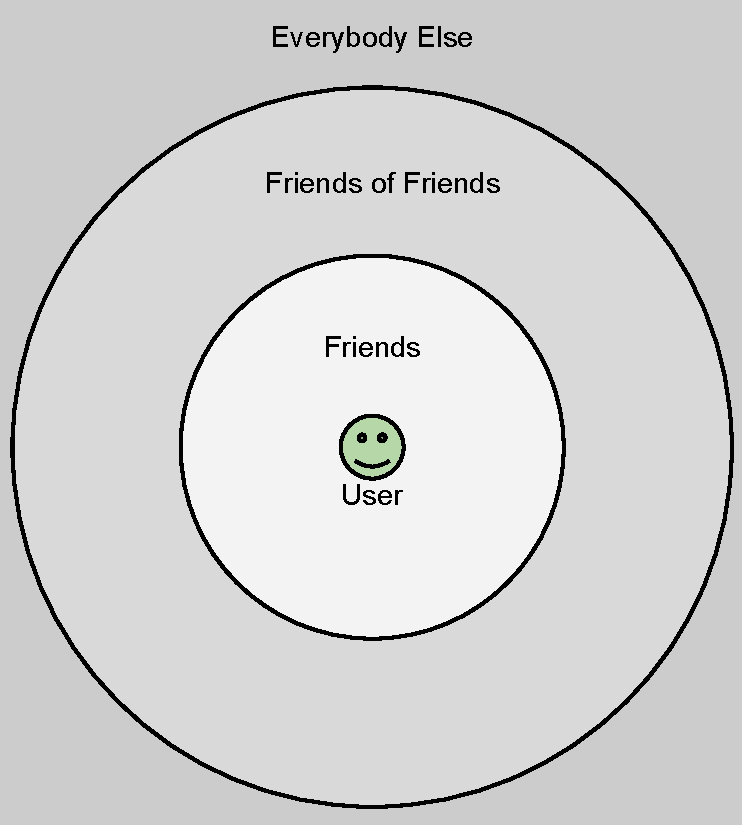
\includegraphics[width=.5\textwidth]{Privacy_Friendship_Circles.pdf}
  \caption{User Centric Social Network Communities. }
  \label{fig:social_circle}
\end{figure}

% modeling social network profiles and items.
Every node $u_i$ in social network $\mathcal{G}$ has $P_i$ number of
features $F_{i}=\{f_{ij}|1\leq j\leq P_i\}$. These
features, in social network, corresponds to the profile items of a
user, e.g. name, date of birth, address, education etc., which are the
identities of user $u_i$ in the social network. Profile items
are basic information for social interaction and can also be used by
social network providers to provide personalized
services such as friends recommendation, search and targetted
advertising.

Usually, social networks require a minimum number of items upon
registration, for example, sex, birthday etc.. And other optional
items can be updated later. Because profile items are carriers of
personal private information, social network sites provide
configuration options for user to change their targetted audience for
each item. For a user $u_i$, we denote the setting of social network
profile item $f_{ij}$ as $s_{ij}$. For example, Facebook provides
settings that include only me, friends only, friends of friends and
everybody from the most conservative to the most open. So for the case
of facebook, we have $s_{ij}\in \{S_{me},S_f,S_{fof},S_{all}\}$. And
we will use these levels of settings in our privacy model.
Although Facebook also provide finer grained privacy setting by
specifying specific users to view a certain profile item, in our model
we ignore this situation and will leave it for future work. The
meaning and corresponding audiences of each privacy settings are
listed in Table \ref{tbl:setting}.

% a table showing the meaning of each privacy level and related
% audiences.
\begin{table}[h]
  \centering
  \begin{tabular}{l|l}
    \toprule
    \textbf{Access Setting} & \textbf{Audiences} \\ \toprule
    Only Me($S_{me}$) & $\mathcal{C}_{USER}$\\ \midrule
    Friends ($S_f$) & $\mathcal{C}_F$ \\ \midrule
    Friends of Friends ($S_{fof}$) & $\mathcal{C}_{FOF}$ \\ \midrule
    Everybody $(S_{all})$ & $\mathcal{C}_{ALL}$ \\ \bottomrule
  \end{tabular}
  \caption{Profile Item Access Setting and Corresponding Audiences.}
  \label{tbl:setting}
\end{table}

\section{The Item Response Theory Model}
In this section, we will have a brief review of the item response
theory(IRT). The original IRT model is only used to model dichotomous
tests, which include only correct or incorrect outcomes. The
polytomous model was proposed to handle cases with multiple outcomes. 

Item Response Theory is a paradigm for the design, analysis, scoring
of tests and questionnaires measuring abilities, attitudes and other
variables. It is based on the idea that the probability of a correct
response to an item is mathematically determined by some parameters of
persons and items. The person parameter is usually called latent
trait, ability or the strength of an attitude. 

The common approach to test the ability of an examinee is to develop a
test consisting a number of items, each item is used to test a certain
ability of interest, the items are dichotomously scored such that
correct answers with get score of ones and zeros for incorrect
answers. The probability that an examinees can correctly answers an
question is determined on the one hand by the ability of the examinee,
and by the item difficulty on the other hand. The ability is denoted
as $\theta$ and the probability of answering an question item correct
with ability $\theta$ is $P(\theta)$. And for a specific test item
$P(\theta)$ will be larger for high ability examinees and lower for
low ability examinees. 

%How to use IRT for test analysis.
\subsection{Application of test analysis of IRT model}
Two general processes are involved for IRT to be used in test analysis.
\begin{enumerate}
\item Test calibration.
  The test calibration stage is used to determine the item
  characteristic curve(ICC) for a specific test item. Alan
  Birnbaum proposed a two stage iterative method with maximum
  likelihood estimation. In one stage the parameters of N items
  in a test are estimated and in the second stage, the ability
  parameters of the M examinees are estimated. These two stages
  are performed iteratively until a stable set of parameter sets
  are obtained. At that point, a test has been calibrated and a
  ability scale metric defined. 

\item Examinee ability prediction with the IRT model.
  The task of this step is to estimate the ability of an
  examinee with a test. Let's suppose a test with N item is
  given a an examinee, and the examinee responses to each of
  these questions resulting in a dichotomous score vector for
  this test. By using the test score as a prior ability of the
  examinee and along with the parameters of each item, we can
  iteratively estimate the ability of an examinee with maximum
  likelihood estimation with the following formula. 
  \[ \hat{\theta}_{s+1} = \hat{\theta}_{s} +
  \frac{\sum_{i=1}^N-a_i[u_i -
    P_i(\hat{\theta}_s)]}{\sum_{i=1}^Na_i^2P_i(\hat{\theta}_s)Q_i(\hat{\theta}_s)
  } \] 
  where $\hat{\theta}_s$ is the estimated ability of the examinee
  within iteration $s$; $a_i$ is the discrimination parameter of item
  $i\in \{1,2,\ldots,N\}$; $u_i$ is the response made by the examinee
  to item $i$; $P_i(\hat{\theta}_s)$ is the probability of item $i$
  under the given item characteristic curve model, at ability level
  $\hat{\theta}$ within iteration $s$; and
  $Q_i(\hat{\theta}_s)=1-P_i(\hat{\theta}_s)$ is the probability of
  incorrect response to item $i$, under the given item characteristic
  model, at ability level $\hat{\theta}$ within iteration $s$. 
  An example is shown shown in figure \ref{fig:predict-ability}.
  \begin{figure}
    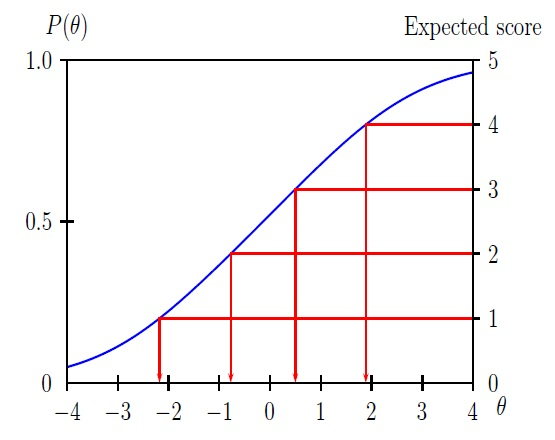
\includegraphics{ability.jpg}
    \caption{Ability estimation using a test with five items.}
    \label{fig:predict-ability}
  \end{figure}
\end{enumerate}

\textbf{The One parameter IRT model} \\
This IRT model has only one parameter $b$, and can be shown as in Eq
\ref{eqn:1pl}. 
\begin{equation}
    P(\theta|b) = \frac{1}{1+e^{-(\theta - b)}}
    \label{eqn:1pl}
\end{equation}

\textbf{The Two parameter IRT model}\\
This model has an ability parameter and a discrimination parameter. 
\begin{equation}
    P(\theta|a,b) = \frac{1}{1+e^{-a(\theta - b)}}
    \label{eqn:2pl}
\end{equation}

\textbf{The Three Parametric Model} \\ 
\begin{equation}
    P(\theta|a,b,c) = c + (1-c)\frac{1}{1+e^{-a(\theta - b)}}
    \label{eqn:3pl}
\end{equation}

\subsection{Concrete example}
\[\begin{array}{ccccc}
  1 & 1 & 1 & 1 & 1 \\
  0 & 1 & 1 & 1 & 1 \\
  0 & 0 & 1 & 1 & 1 \\
  0 & 0 & 0 & 1 & 1 \\
  0 & 0 & 0 & 0 & 1 
\end{array}
\]
\section{Exploring Perceived Privacy Risk}
% describe real privacy risk and perceived privacy risk.
% why do we want to study perceived privacy risk.
% how do we do that? Procedure/algorithm, the use of IRT model to
% derive latent variables.
% users' settings is a tradeoff between risk and benefit - how to
% incorporate this tradeoff into the model.
% what is social network works and how to get it from data?
Risks and attacks of online social network reflect the potential
damage to social network users. And users are learning, they start to
make careful decisions about what information to put online under
which circumstances, at the same time, more and more people are
changing to a more restrictive privacy setting \cite{socialnet:setting}.
Usually, social network users will have risk considerations in
mind when disclosing their private information
on the social network. And it has been shown
\cite{privacy:paradox:revisit} that stronger privacy
concerns resulted in more restrictive profile settings.

% defining perceived risk.
\begin{simondef}
Perceived risk is the direct reflection of
user's opinion on how sensitive a specific profile item is to
him/her-self. And this opinion will guide user make privacy settings
on social network.
\end{simondef}

\section{Modeling Realized Privacy Risk}
% argument: privacy risk is not realized until the user exposes the
% profile item to other users. The user setting (F,FoF, E) determines
% different levels of realized privacy risk.
% a Bayesian model: expected realized privacy risk = privacy risk
% measure * Prob(user attacks)
% Prob(user attacks) =
% case 1. Expose to F only. sum Prob(friend i attacks)
% case 2. Expose to FoF. Sum Prob(friend i attacks) + sum Prob(FoF i attacks)
% case 3. Expose to everybody. Sum Prob(friend i attacks) + sum
% Prob(FoF i attacks) + sum Prob(everybody else i attacks)

% Prob(user attacks) = Prob(user attacks|user visits your profile
% item)* prob(user visits).

% prob(user visits) is defined by the network structure
% i.e., prob(friend i visits) is determined by how many friends that
% friend i has (n_{f_i}) and make it uniform (1/ n_{f_i})
% prob (fof i visits) = \sum prob(fof i visits neighbor j) prob (from
% neighbor j to you)
% prob (everybody else visits) = prob(search your name) + prob(find
% you through the f/fof/fofof/… links)
% analyze each probs and you may make assumption on some probs such as
% prob(search your name).
% The realized social network privacy.
\subsection{Realized Social Network Privacy}
% definition of privacy realized upon ....
\begin{simondef}
The social benefits and/or social risks
of user $u_i$ are realized when user $u_j, j\neq i$ visits the profile
item $f_{ij}$ of $u_i$, and we call the the social network privacy of
$u_i$ is realized upon event $e_{u_j\rightarrow u_i}$.
\end{simondef}

% probabilistic realization of privacy.
We define the probability that the profile item $f_{im}$ of user $u_i$
is visited by user $u_j$ as $p_{jim}$.

Use $b_{jim}$ to denote benefit of $u_j$ access profile item $f_{im}$
of $u_i$.

% defining realized social benefits.
The realized benefit of user $u_i$ is defined as:

\[ \mathcal{B}_i = \alpha_i \sum_{m\in \{1,2,\ldots,N_i\}}\sum_{j\in
  \mathcal{C}}b_{jim}\times p_{jim} \]

where $\alpha_i$ is parameter specific to each user, $N$ is the number
of items that user $u_i$ has, and $\mathcal{C}\in \{\mathcal{C}_{USER},
\mathcal{C}_{F}, \mathcal{C}_{FOF} \mbox{ and } \mathcal{C}_{ALL}\}$
is the community of friendship.

% defining realized risk.

The realized risk of user $u_i$ is defined as:

\[ \mathcal{R}_i = \beta_i \sum_{m\in \{1,2,\ldots,N_i\}}\sum_{j\in
  \mathcal{C}} r_{jim}\times p_{jim} \]

where $\beta_i$ is the risk factor for user $u_i$, $r_{jim}$ is the
risk when $u_j$ visits profile item $f_{im}$ of user $u_i$, and
$p_{jim}$ is the probability of user $u_j$ visits profile item
$f_{im}$ of user $u_i$.

% defining the probability of visiting.
For every friend $u_j,j\in \{1,\ldots,N_i\}$ of user $u_i$, the
probability that $u_j$ visits $u_i$ is determined by the number of
friends $u_j$ has. And by assuming the simplest equal probability
model we have $p_{ji}=\frac{1}{N_j}$, where $N_j$ is the number of
friends that $u_j$ has.

For every friend of friend $u_j,j\in \{1,\ldots,N_i\}$ of
user $u_i$, the probability that $u_j$ visits $u_i$ is determined by
the number of friends of friends $u_j$ has. And by assuming the simplest equal
probability model we have $p_{ji}=\frac{1}{\sum_{k=1}^{N_j}N_k}$,
where $N_k$ is the number of friends of $u_j$'s friend $u_k$ has.

\subsection{Deriving Benefit $b_{jim}$ From Perceived Benefit}
Social network benefit should be a perception of $u_i$ about the
benefit he can get by setting a certain privacy level. So, it is user
specific. So, $b_{jim} = o_{jim}$, where $o_{jim}$ is the observed
benefit when $u_j$ visits profile item $f_{im}$ of $u_i$, which is
actually the specific setting of privacy level for profile item
$f_{im}$ of user $u_i$.

\subsection{Deriving Risk $r_{jim}$ From Perceived Risk}
Social network risk $r_{jim}$, is a natural property of a profile item
$f_{m}$, it is the nature of the profile item, for example, some
profile items are more risky than others in nature. Example,
\emph{phone number} is more risky than \emph{education}. So, by this
defnition, we can rewrite $r_{jim}$ as $r_m$. We say that profile item
$f_m$ is more \emph{risky} when more people set this item to be a more
restrictive privacy level.

% A linear model to derive profile item risk from observed privacy
% setting.
By using linear model, assign integer values to each privacy level
$\mathcal{S}\in \{\mathcal{S}_{me}=1, \mathcal{S}_{f}=2,
\mathcal{S}_{fof}=3, \mathcal{S}_{all}=4\}$, we can define $r_m$ as
mean value of aggregated privacy level settings.
\[ r_m = \frac{1}{N} \sum_{i=1}^No_{im} \]
where $o_{im}$ is observed privacy setting of profile item $f_{im}$
of $u_i$.

% Exponetial model
\subsection{Item Response Theory (IRT) model}
% background of the item response theory. 
Item response theory was first used in psychometrics as a theory
to design, analyze tests. The goal is the measure the abilities of
examinees. 

The IRT model assumes each examinee is characterized by an ability
level $\theta$, and every question is characterized by two parameters:
difficulty $\beta$ and discrimination $\alpha$. Intuitively, examinee
ability can be measured by the number of questions answered correctly
in a given test, 
the more one can answer questions correctly, the higher ability
one has. And item difficulty has the similar measurements, the fewer
people who can answer a question correctly, the more difficult the
question is. By indentifying the item difficulty as a latent variable,
the IRT model measures the probability that an examinee $j$ answers an
item $i$ correctly by 
\begin{equation}
  P_{ij}(\theta_j) = \frac{1}{1+e^{\alpha_i(\theta_j-\beta_i)}}
\end{equation}
So, probability $P_{ij}$ is determined by parameter $\theta_j$ and
latent variables $\alpha_i$ and $\beta_i$. With given $\alpha_i$ and
$\beta_i$, the plot of $\theta_j$ and $P_{ij}$ is called item
characteristic curve (ICC). As each item has its own latent variable,
they can also be characterized by different ICCs. 

% TODO. 
% property of the ICC, what is the meaning of $\alpha$ and $\beta$. 
Figure \ref{} shows ICCs of two items item1 and item2 with fixed
$\alpha$ and $\beta_1 > \beta_2$. From the figure, we can see that
with given probability level, item2 has higher probability to be
answered correctly. On the other hand, figure \ref{} shows two ICCs
with same $\beta$ for two items and $\alpha_1 > \alpha_2$. We can see
that if ability is higher than mid-point, item1 has higher probability
to be answered correctly, and if the ability level is lower than
mid-point, item2 has is easier than item1. We say that item1 has
higher discrimination power. 

\begin{figure}[h]
  \centering
  \includegraphics{} 
  \includegraphics{} 
\end{figure}

% mapping from IRT model to our privacy model. 
Social network provides users with choices to configure their privacy
preferences for their profile items. With regard to the IRT model, we
map examinees to social network users, and test questions to user's
profile items. The ability of an examinee corresponds to the attitude
of user towards the social network privacy. In our model, we assume
that user's setting of of their social network privacy item is a
reflection of both his/her sense of benefit from the social network
as well as the risks within the social network. When a user considers
about setting a profile item to a certain privacy level, he usually
leverages the benefits and the risks by doing this. If he thinks that
the benefit is higher than risk, he will set it to a higher level, and
to a lower level if the perspected risk is higher than benefit. 

% privacy setting change statistics. 

% perception of risk vs. benefits.
% quantitative leverage between benefits and risks. 

% how to obtain the data from facebook.
In this section, we are going to discuss our method to obtain profile
item visibility data from facebook. The data we are exploring are from
my friends and my friends of friends. So, we denote the account for my
friends as my account. 

As of the time of crawling data from facebook, my account has around
135 friends and 5730 friends of friends. We first build the social
graph for my friends and my friends of friends. And then crawl the
data related to the user's profile items, such as birth date, hometown
etc. What we get from this crawl is the binary visibility of user's
profile item with regard to my account. We can not make decision to 
which privacy level the user has set for a specific profile item. In
order to do this, we create a new facebook account, no friends, which
we call nobody account, and then we use this account to crawl the
social graph we stored for my friends and friends of friends. By
combining the binary visibility data for my account and nobody
account, we can infer multi-level visibility settings for users'
profile items. 

% basic data description.
After cleaning and removing all the error data, we get 99 user
profile item settings which are friends of my account and 3798 user
profiles item settings for my friends of friends data. 

% rules to infer multi-level visibility from binary visibility data. 
With the binary visibility settings from two users, we used inference
rules (which are shown in table \ref{tbl:f_vis_setting} and
\ref{tbl:fof_vis_setting}) to obtain the multi-level privacy
settings. In the binary data, 
we use 'Y' if the item is visible to the crawling account and 'N'
otherwise. For the case of facebook, there are four visibility
levels \footnote{There is another level, which allows user to select
  specific users to see a specific item, but we ignore this part in
  our paper.}: user only (U), friends only (F), friends of friends
(FOF) and everybody (E). And we use 'ERROR' to denote impossible cases. 

For friends data, we have: \\
\begin{table}[h]
  \centering
  \begin{tabular}{l|l}
    \toprule 
    \textbf{My Account} & \textbf{Nobody Account} & Visibility \\ 
    \toprule
    Y & Y & E \\ \midrule 
    Y & N & F/FOF \\ \midrule 
    N & Y & ERROR \\ \midrule 
    N & N & U \\ \midrule 
  \end{tabular}
  \caption{Profile Item Access Setting and Corresponding Audiences.}
  \label{tbl:f_vis_setting}
\end{table}

And for friends of friends data, we have: \\ 
\begin{table}[h]
  \centering
  \begin{tabular}{l|l}
    \toprule 
    \textbf{My Account} & \textbf{Nobody Account} & Visibility \\ 
    \toprule
    Y & Y & E \\ \midrule 
    Y & N & FOF \\ \midrule 
    N & Y & ERROR \\ \midrule 
    N & N & U/F \\ \midrule 
  \end{tabular}
  \caption{Profile Item Access Setting and Corresponding Audiences.}
  \label{tbl:fof_vis_setting}
\end{table}

In our visibility inference rule, when a profile item is visible to my
account while invisible to nobody account, we can not make decision
whether the privacy setting for this item is friends only or friends
of friends. And similar for friends of friends data, when both my
account and nobody account is binary invisible, we can not make
decision whether the privacy setting is user only or friends only. 

% how to handle this situation? 
In order to handle this problem 

%%%%%%%%%%%%%%%%%%%%%
% basic description of item settings data. 
% setting change statistics. 
We say that the privacy setting for an item was changed if it is
different from the default setting. 

We expect that, when fixed risk levels $\beta_j$, the higher
$\alpha_i$, the harder to get satisfied; and when fixed $\alpha_i$,
less risky profile items can be easily satisfied. Figure \ref{fig:irta}
and Figure \ref{fig:irtb} have better illustration of these
expectations.
\begin{figure}[H]
  \centering
  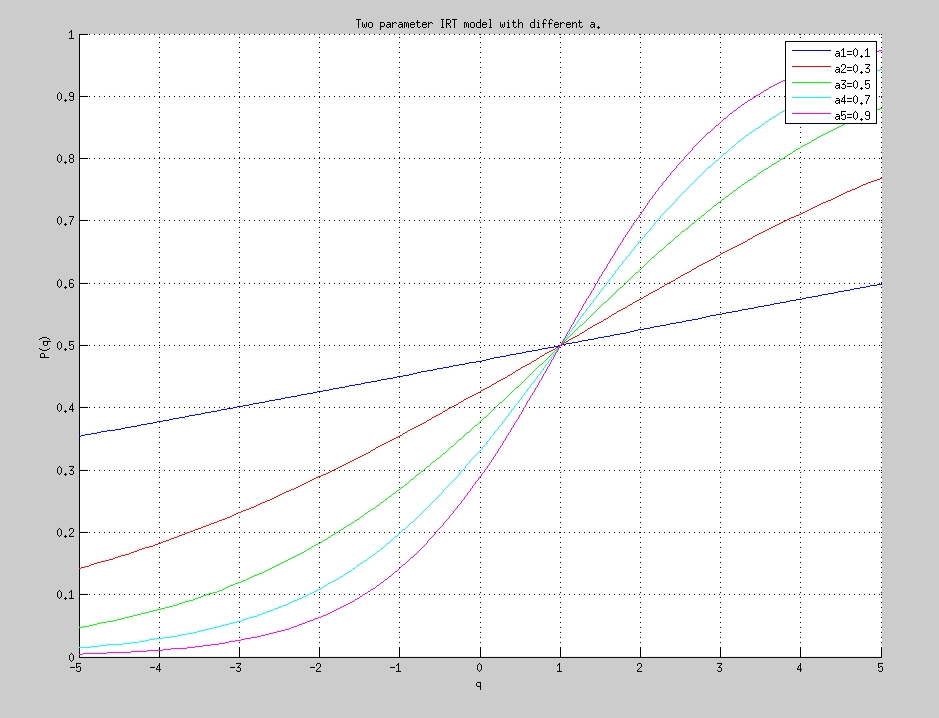
\includegraphics[width=.7\textwidth]{IRT-a.jpg}
  \caption{Satisfaction With different perception level.}
  \label{fig:irta}
\end{figure}

\begin{figure}[H]
  \centering
  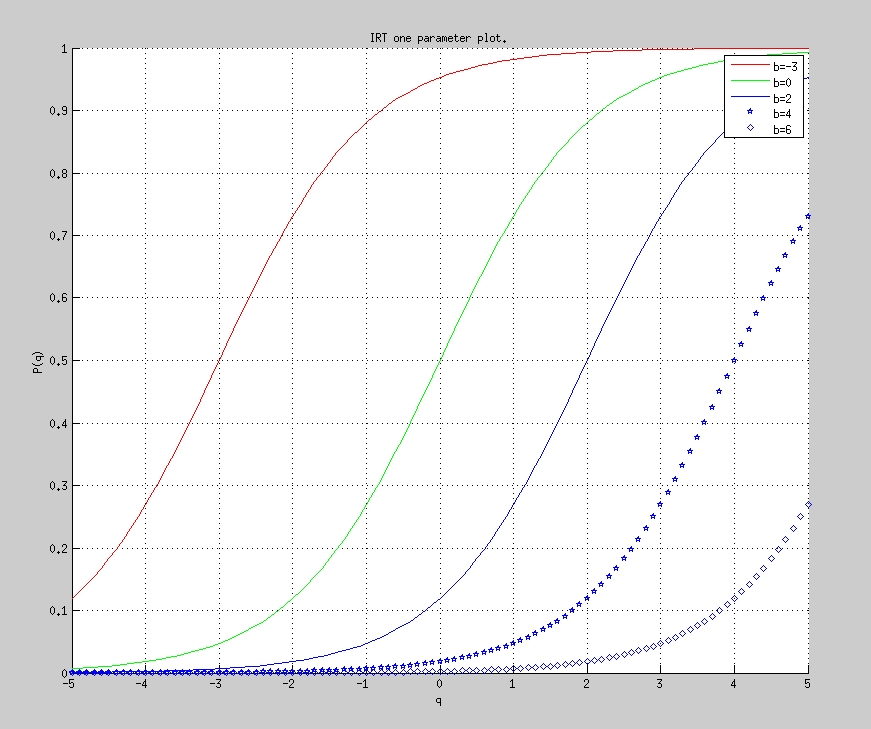
\includegraphics[width=.7\textwidth]{IRT-b.jpg}
  \caption{Satisfaction With different profile risk level.}
  \label{fig:irtb}
\end{figure}

And we can use optimization techniques to estimate parameters of
benefit expectation factor $\alpha_i$ and risk $\beta_j$.

\section{Experiments}
% describe how you derive the perceived privacy risk with the data
% from facebook.
% use some materials in your previous reports.
Facebook is one of the largest social networking sites, with more than
800 million users\cite{facebookwiki} and it provides a very
comprehensive privacy configuration page that let users make their
privacy choices. We derive the privacy settings by crawling user's
facebook pages using two accounts, one is my account which has about 100
friends and the other is nobody's account with no friends to represent
a random user on facebook.

\subsection{Deriving User's Privacy Settings}

\section{Related Work}
% summarize the importance of privacy setting in one paragraph
% summarize the attacks in one paragraph
% summarize privacy setting problem in one paragraph

% Privacy research.
In recent years, research community has been trying hard to deal with
privacy issues of online social networks, related topics include
spamming and phishing \cite{twitter-spam, SN-explore-spam,
SN-automated-cheap-spam, social-spam-detection, video-spam-youtube},
attack analysis \cite{neighborhood-attack, 1658958,
group-deanonymization-attack, anony-link-attack,
identity-theft-attack, sybil-attack, 1608132} etc., which are also
directly related to traditional web privacy and security. Fang et
al. \cite{privacy-wizard} proposes a classification model to help
social network users automate the privacy related settings. Social
network privacy control is also considered an access control
problem. Carminati et al. \cite{crypto-collaborative-ac,
rule-based-ac} propose client-based semi-decentralized access control
model, access is granted based on the attestation of access
authorization by the access requestor. Mohd et
al. \cite{Anwar_visualizingprivacy} proposes a reflective policy
assessmenst method based on visualization to help user understand the
implications of access control policies. Another research branch
related to social network privacy is related to the social network
platform, which targets privacy risks by third party application and
social network providers. Adrienne et
al. \cite{Felt08privacyprotection} addresses the privacy risks
associated with social network APIs through proxy. Singh et
al. \cite{xbook-social-platform} propose an information flow model to
control what untrusted applications can do with the information they
receive.

% Privacy attacks.
Spamming, phishing and attack of social network sites is another topic
that is related with
privacy. Kyumin Lee et al. \cite{social-spammer-machine-learning},
Stringhini et al. \cite{SN-detect-spam}, Gao, Hongyu et
al. \cite{SN-spam-campaigns} and Huber, Markus et
al. \cite{SN-explore-spam}. It is found that the
identified spam data contains contents that are strongly correlated
with observable profile features. Tom Jagatic et al. \cite{social-phishing}
studied phishing attacks by using the publicly available personal
information from social networks. They find that the phishing attack
was easy and effective with a success rate of $72\%$. Bilge, Leyla et
al.\cite{identity-theft-attack} studied identity
theft attacks, and find that existing users of OSN can be
compromised, and their identity can be used to request friendship with
other cloned victims. Lars Backstrom et al. \cite{anony-link-attack}
and Gilbert Wondracek et al. \cite{group-deanonymization-attack}
deanonymization of private data can cause severe privacy breach in the
context of anonymized data publication. Besides, social network
friendship can also bring privacy threats to social network
users. \cite{user-interaction-social-link} and
\cite{neighborhood-attack} studied the risks that social interaction
and frienship can bring.

% privacy setting problems.
With the increasing concern of users and various social network
incidents, social network sites are pressed to provide more and more
finer grained privacy control configurations. For example, facebook
has been refining their privacy setting over time. But on the other
hand, although user awareness of social network users are increasing,
and more and more users change their privacy settings. It is hard for
them to fully understand and configure these settings. Fang Lujun et
al. \cite{privacy-wizard} propose a machine learning based method to
help users automatically make the settings.

\bibliographystyle{unsrt}
\bibliography{privacy}

\end{document}
